
\documentclass{unswmaths}
\usepackage{mathtools}
\usepackage{unswshortcuts}
\usepackage{fullpage}
\usepackage{float}
\usepackage{pgfplots}

\author{Adam J. Gray}
\studentno{3329798}
\subject{Biomathematics}
\title{Assignment 1}


\begin{document}

\unswtitle

\section*{Question 1}
\subsection*{a}
	$ F $ is a linear combination of $ N $ and $ \frac{dN}{dt} $. This means that the larger the population is the more demand for the food there is. It also means that the faster the populations is growing, the more demand for food there is which would make sense because cell division could require \emph{more resources}.
\subsection*{b}
	\begin{align*}
		\frac{dN}{dt} &= rN \frac{T - \left(c_1N + c_2\frac{dN}{dt}\right)}{T} \\
		\frac{dN}{dt} \left( 1 + \frac{rc_2N}{T}\right) &= rN\left(1 - \frac{c_1N}{T} \right) \\
		\frac{dN}{dt} &= rN \left( \frac{\frac{T}{c_1} - N}{\frac{T}{c_1} + \frac{rc_2N}{c_1}} \right) \\
			&= rN \left( \frac{K - N}{K + aN}\right)
	\end{align*}
	where $ K = \frac{T}{c_1} $ and $ a = \frac{rc_2}{c_1} $.
\subsection*{c}
	Let $ f(N) = rN\left( \frac{K-N}{K+aN} \right) $ thus $ f(N) = 0 \Longrightarrow N^* = 0, N^* = K $.
	\begin{align*}
		f'(N) = r \left( \frac{K-N}{K+aN} \right) + rN \left( \frac{-(K+aN) - (K-N)a}{(K+aN)^2}\right)
	\end{align*}
	and
	\begin{align*}
		f'(0) &= r > 0 \\
		f'(K) &= \frac{-r}{a+1} < 0
	\end{align*}
	thus the steady states are $ N = 0 $ and $ N = k $ and they are unstable and stable respectively.
\section*{Question 2}
\subsection*{a}
	\begin{align*}
		\frac{dx}{dt} = 0 &\Longrightarrow 0.2x\left( 1 - \frac{x}{3} \right) = 0 \\
			& \Longrightarrow x^* = 0, 3
	\end{align*}
	So the steady states of the system are $ x^* = 0 $ and $ x^* = 3 $.
\subsection*{b}
	\begin{align*}
		\frac{dx}{dt} &= 0.2x\left( 1 - \frac{x}{3} \right) \\
		\int \frac{dx}{x(3-x)} &= \frac{1}{15} \int dt \\
		\int \frac{dx}{3x} + \int \frac{dx}{3(3-x)} &= \frac{1}{15} \int dt \\
		\frac{1}{3} \ln(x) - \frac{1}{3} \ln(3-x) &= \frac{t}{15} + C \\
		\ln \left( \frac{x}{3-x} \right) &= \frac{t}{5} + B \\
		\frac{x}{3-x} &= \exp(\frac{t}{5} + B) \\
		x &= \frac{3\exp(\frac{t}{5} + B)}{1 + \exp(\frac{t}{5} + B)}
	\end{align*}
	As $ x(0) = x_0 $
	\begin{align*}
		B &= \ln \left( \frac{x_0}{3-x_0} \right)
	\end{align*}
	and so
	\begin{align*}
		x = \frac{3 x_0 \exp(\frac{t}{5})}{3 + x_0 (\exp(\frac{t}{5}) - 1)}.
	\end{align*}
\subsection*{c}
	The steady states of the population are
	$ x^* = 0 $ and $ x^* = 3 - 15E $. Note that the second steady state is a function of $ E $ and for a sustainable yield we would require $ E < \frac{1}{5} $ so that the steady state is positive.
	
\subsection*{d}
	As per the last section the maximum sustainable yeild is $ E = \frac{1}{5} $.

\section*{Question 3}
Let $ H : [0, \infty) \lra \mathbb{R} $ be defined as
\begin{align*}
    H(t) = 
    \begin{cases}
        h & t \mod 12 \leq T \\
        0 & \text{ otherwise }
    \end{cases}
\end{align*}
where $ h $ is the harvesting quantity. 
Then assuming that there are no other population limiting factors, the governing equation would be
\begin{align*}
    \frac{dF}{dt} = rF - H(t)
\end{align*}
where $ F(t) $ is the population of fish at time $ t $ (months) and $ r $ is the population growth rate in fish per month.

\section*{Question 8}
\subsection*{a}
    \begin{align*}
        \underbrace{\frac{dx}{dt}}_{animals\cdot km^{-2} \cdot day^{-1}} = \underbrace{a}_{day^{-1}}\underbrace{x}_{animals \cdot km^{-2}} - \underbrace{b}_{animals^{-1} \cdot km^{2} \cdot day^{-1}}\underbrace{xy}_{animals^{2} \cdot km^{-4}} \\
        \underbrace{\frac{dy}{dt}}_{animals\cdot km^{-2} \cdot day^{-1}} = -\underbrace{c}_{day^{-1}}\underbrace{y}_{animals \cdot km^{-2}} + \underbrace{d}_{animals^{-1} \cdot km^{2} \cdot day^{-1}}\underbrace{xy}_{animals^{2} \cdot km^{-4}} \\
    \end{align*}
\subsection*{b}
     \begin{align*}
        \frac{dx(t)}{c} &\sim \frac{animals^{-1} \cdot km^2 \cdot days^{-1} animals \cdot km^{-2}}{days^{-1}} &\sim unitless \\
        \frac{by(t)}{a} &\sim \frac{animals^{-1} \cdot km^2 \cdot days^{-1} animals \cdot km^{-2}}{days^{-1}} &\sim unitless \\
        at &\sim days^{-1} \cdot days &\sim unitless \\
        \frac{c}{a} &\sim \frac{days^{-1}}{days^{-1}} &\sim unitless
     \end{align*}
\subsection*{c}
    Chain rule:
    \begin{align*}
        \frac{du}{d\tau} = \frac{du}{dt} \frac{dt}{d\tau} = \frac{d}{ca}\frac{dx}{dt} \\
        \frac{dv}{d\tau} = \frac{dv}{dt} \frac{dt}{d\tau} = \frac{b}{a^2} \frac{dy}{dt} \\
    \end{align*}
    Subbing in:
    \begin{align*}
        \frac{du}{d\tau} &= \frac{d}{ca} \left( ax + bxy \right) \\
            &= \frac{d}{ca} \left( \frac{ac}{d} u + \frac{bca}{db} v\right)u \\
            &= u(1-v) \\
        \frac{dv}{d\tau} &= \frac{d}{a^2} \left( -cy + dxy \right) \\
            &= \frac{d}{a^2} \left( \frac{-ca}{b} v + d\frac{bca}{db} vu\right) \\
            &= \frac{c}{a} v\left(u - 1\right) \\
            &= \alpha v(u - 1)
    \end{align*}
    Equilibrium points:
    \begin{align*}
        \frac{du}{d\tau} = u(1-v) = 0 \Longrightarrow  u = 0 \text{ or } v = 0 \\
        \frac{dv}{d\tau} \alpha v(u-1) = 0 \Longrightarrow v = 0 \text{ or } u = 1 \\
    \end{align*}
    For equilibriums $ u = 0 \Longrightarrow v = 0 $ and $ v = 1 \Longrightarrow u = 0 $.
    Thus equilibriums are at $ (0,0) $ and $ (1,1) $.
\subsection*{d}
    \begin{align*}
        \frac{dv}{du} &= \frac{dv}{dt} \frac{dt}{du} \\
            &= \frac{\alpha v(u-1)}{u(1-v)}
    \end{align*}
    Integrating:
    \begin{align*}
        \int \frac{(1-v)}{v}dv &= \alpha \int \frac{(1-u)}{u} du \\
        \ln(v) - v &= \alpha \ln(u) - \alpha u + C \\
        \ln(v) - v &= -\ln(u^\alpha) + \alpha u  + C \\
        \ln(u^\alpha v) - v -\alpha u &= C
    \end{align*}
\subsection*{f}
    Differentiating:
    \begin{align*}
        \frac{dC}{du} &= \frac{1}{u^\alpha v} ( \alpha u^{\alpha-1} v ) - \alpha \\
        \frac{dC}{dv} &= \frac{1}{u^\alpha v} - 1
    \end{align*}
    Stationary points:
    \begin{align*}
        \frac{1}{u^\alpha v} ( \alpha u^{\alpha-1} v ) - \alpha = 0 \Longrightarrow u = 1 \\
        \frac{1}{u^\alpha v} - 1 = 0 \Longrightarrow u^\alpha v = 1 \Longrightarrow v = 1
    \end{align*}
    Only one stationary point so this \emph{must} be the maximum. 
    
    Maximum at $ (1,1) $ with value $ 1 + \alpha $ (by simple subsitituion).
\section*{Question 9}
\subsection*{a}
\begin{figure}[H]
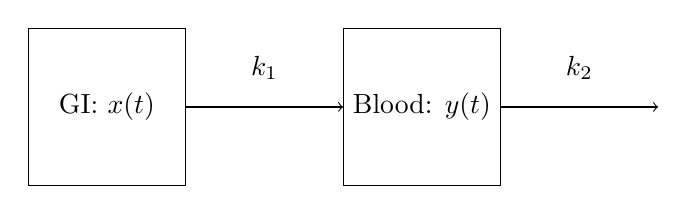
\begin{tikzpicture}
    \draw (0,0) -- (0,2) -- (2,2)  -- (2,0) -- (0,0);
    \draw[->] (2,1) -- (4,1);
    \draw (4,0) -- (4,2) -- (6,2) -- (6,0) -- (4,0);
    \draw[->] (6,1) -- (8,1);
    \draw (1,1) node {GI: $ x(t) $};
    \draw (5,1) node {Blood: $ y(t) $};
    \draw (3,1.5) node {$k_1$};
    \draw (7,1.5) node {$k_2$};
\end{tikzpicture}
\end{figure}

The system of differential equations is given by
\begin{align*}
    \left( \begin{array}{c} \frac{dx}{dt} \\ \frac{dy}{dt} \end{array}\right) &= \left[ \begin{array}{cc} -k_1 & 0 \\ k_1 & -k_2 \end{array} \right] \left( \begin{array}{c} x(t) \\ y(t) \end{array}\right)
\end{align*}
along with the inital conditions
\begin{align*}
    x(0) &= A \\
    y(0) &= 0 
\end{align*}
\subsection*{b}
Let
\begin{align*}
   B := \left[
        \begin{array}{cc}
            -k_1 & 0 \\
            k_1 & - k_2
        \end{array}
        \right].
\end{align*}
It is clear to see that this has eigenvalues $ \lambda_1 = -k_1 $ and $ \lambda_2 = -k_2 $. Simple computations show that the corresponding eigenvectors are
\begin{align*}
    \mathbf{v}_1 &= \left( \begin{array}{c} 1/k_1 \\ 1/(k_2-k_1) \end{array}\right) \\
    \mathbf{v}_2 &= \left( \begin{array}{c} 0 \\ 1 \end{array}\right)  
\end{align*}
and so the general solution to the system of differential equations is
\begin{align*}
    \left( \begin{array}{c} x(t) \\ y(t) \end{array} \right) = \alpha \left( \begin{array}{c} 1/k_1 \\ 1/(k_2 - k_1) \end{array}\right) e^{-k_1 t} +  \beta \left( \begin{array}{c} 0 \\ 1 \end{array}\right) e^{-k_2 t}.
\end{align*}
By applying the initial conditions we get that system of equations
\begin{align}
    \alpha \left( \begin{array}{c} 1 / k_1 \\ 1 / (k_2 - k_1) \end{array} \right) + \beta \left( \begin{array}{c} 0 \\ 1 \end{array} \right) = \left( \begin{array}{c} A \\ 0 \end{array}\right)
\end{align}
which gives us that $ \alpha = k_1 A $ and $ \beta = -k_1 A / (k_2 - k_1 ) $.
So the solutions look like
\begin{figure}[H]
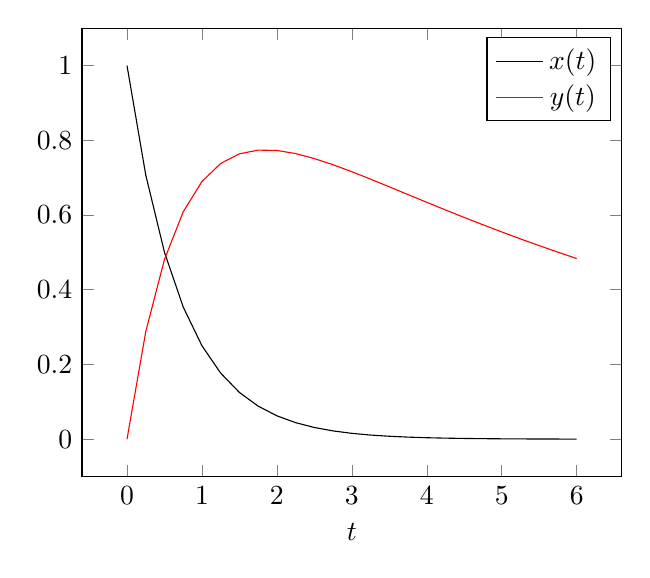
\begin{tikzpicture}
    \begin{axis}[
        xlabel = $t$
    ]
    \addplot[domain=0:6] {exp(-1.386*x};
    \addplot[domain=0:6,color=red] {-1.1111 * exp(-1.386 * x) + 1.1111 * exp(-0.1386 * x)};
    \addlegendentry{$x(t)$}
    \addlegendentry{$y(t)$}
    \end{axis}
\end{tikzpicture}

Decongestant levels quickly drop in the GI tract but they build up quickly in the blood and are slow to clear from the blood.
\end{figure}
\end{document}
